%!TeX encoding=utf8
%%%%%%%%%%%%%%%%%%%%%%%%%%%%%%%%%%%%%%%%%%%%%%%%%%%%%%%%%%%%%%%%%%%%%%%%%%%%%%%%
% Vorlage für mit LaTeX formatierte Versuchsberichte im Physikpraktium
%%%%%%%%%%%%%%%%%%%%%%%%%%%%%%%%%%%%%%%%%%%%%%%%%%%%%%%%%%%%%%%%%%%%%%%%%%%%%%%%
% Diese Datei steht unter der Lizenz CC0 1.0 . Sie darf kopiert, verändert
% und weitergegeben werden. Zu den Details siehe
% https://creativecommons.org/publicdomain/zero/1.0/deed.en
%%%%%%%%%%%%%%%%%%%%%%%%%%%%%%%%%%%%%%%%%%%%%%%%%%%%%%%%%%%%%%%%%%%%%%%%%%%%%%%%

\documentclass[ngerman]{scrartcl}

\newcommand{\authA}{*Author1*}
\newcommand{\authB}{*Author2*}
\newcommand{\grpnr}{*Grp.-Nr.*}

%%%%%%%%%%%%%%%%%%%%%%%%%%%%%%%%%%%%%%%%%%%%%%%%%%%%%%%%%%%%%%%%%%%%%%%%%%%%%%%%
% Vorspann für mit LaTeX formatierte Versuchsberichte im Physikpraktium
%%%%%%%%%%%%%%%%%%%%%%%%%%%%%%%%%%%%%%%%%%%%%%%%%%%%%%%%%%%%%%%%%%%%%%%%%%%%%%%%
% Diese Datei steht unter der Lizenz CC0 1.0 . Sie darf kopiert, verändert
% und weitergegeben werden. Zu den Details siehe
% https://creativecommons.org/publicdomain/zero/1.0/deed.en
%%%%%%%%%%%%%%%%%%%%%%%%%%%%%%%%%%%%%%%%%%%%%%%%%%%%%%%%%%%%%%%%%%%%%%%%%%%%%%%%


% Optionen für die Dokumentenklasse scartcl von KOMAscript.
\KOMAoptions{
	DIV=11,
	BCOR=0mm,
	paper=a4,
	fontsize=12pt,
	parskip=half,
	twoside=false,
	titlepage=false
}

% Papierformat: DIN-A4, mit wenig Rand
\usepackage[
	a4paper,
	left=20mm,
	right=20mm,
	top=23mm,
	bottom=15mm,
	includefoot,
	footskip=8mm
	]{geometry}

% Zeilenabstand, andere Werte: onehalfspacing, doublespacing
\usepackage[singlespacing]{setspace}

% Definition der Kopf- und Fußzeile
\usepackage[headsepline,automark]{scrlayer-scrpage}
\clearpairofpagestyles
\setlength{\headheight}{2.5\baselineskip}
\setlength{\footheight}{1\baselineskip}
\ihead[]{
\includegraphics[width=4cm]{Images/ap-logo_bw.pdf}}
\chead[]{\authA \\ \authB}
\ohead[]{Datum: \today \\ Gruppe:~\grpnr}
\ofoot[]{\pagemark}

%---Language and umlauts
\usepackage[utf8]{inputenc}       % UTF-8 Kodierung - ä, ö, ü, ß direkt eingeben
\usepackage[ngerman]{babel}                      % Neue deutsche Rechtschreibung
\usepackage[expansion=true, protrusion=true]{microtype} % Bessere Silbentrennung

% Formelsatz
\usepackage{amsmath}		% Mathematik-Umgebungen - z.B. align
\usepackage{amsthm}		% Umgebung "theorem"
\usepackage{amsfonts}	% Schriften
\usepackage{amssymb}		% Symbole
\usepackage{upgreek}		% Griechische Sonderzeichen z.B. \upmu

% Einheiten
\usepackage{siunitx}
\sisetup{
	locale = DE,
	separate-uncertainty,
	range-units = brackets,
	list-units = single,
	per-mode=fraction
}

% Bilder und Tabellen
\usepackage{graphicx}			% Bilder als PDF einbinden
\usepackage{epstopdf}			% Bilder im EPS-Format
\usepackage{caption}				% Unterschriften für Bilder und Tapellen
\usepackage{booktabs}			% Zusätzliche Schönheitslinien für Tabellen
\usepackage{multirow}			% Mehrere Felder in einer Tabelle zusammenfassen
\usepackage[table]{xcolor}		% Für farbig unterlegte Tabellenzeilen
  \definecolor{lightgray}{gray}{0.9}
  \rowcolors{1}{}{lightgray}	% jede zweite Zeile in einer Tabelle leicht grau


% Positionierung von Bildern und Tabellen
\usepackage{float}				% Option 'H', also "hier-egal-wie-das-aussieht"
\usepackage[section]{placeins}	% Platzierung spätestens am Ende eines Kapitels
\renewcommand{\floatpagefraction}{.75}	% standard: .5
\renewcommand{\textfraction}{.1}			% standard: .2
\renewcommand{\topfraction}{.8}			% standard: .7
\renewcommand{\bottomfraction}{.5}		% standard: .3
\setcounter{topnumber}{3}				% standard: 2
\setcounter{bottomnumber}{2}				% standard: 1
\setcounter{totalnumber}{5}				% standard: 3

\usepackage{caption}
\captionsetup[figure]{name=Abbildung,format=plain}
\captionsetup[table]{name=Tabelle,format=plain}

\usepackage{copyrightbox}		% Nachweis der Bildquelle

% Schrift für die Bildquelle
\makeatletter
\renewcommand{\CRB@setcopyrightfont}{%
\usefont{T1}{cmr}{m}{n}\fontsize{10}{10}\selectfont }
\makeatother


% Hyperlinks
\usepackage{hyperref}
\hypersetup{
	colorlinks=true,
	breaklinks=true,
	citecolor=darkgray,
	linkcolor=darkgray,
	menucolor=red,
	urlcolor=cyan,
	bookmarksopen=false,
	bookmarksopenlevel=0,
	plainpages=false,			% zur korrekten Erstellung der Bookmarks
	hypertexnames=false			% zur korrekten Erstellung der Bookmarks
}

\usepackage{pdfpages} 		% Einfügen von Vollseiten-PDFs (z.B. das Deckblatt)
\pdfminorversion=7			% Das Deckblatt-Formular ist ein PDF, version 1.7
\usepackage{csquotes}		% Zitate

% Literaturverzeichnis
\usepackage[style=alphabetic,sorting=ynt,backend=biber]{biblatex}

% Eine Abkürzung, die Computerbefehle im Fließtext mit einer Mono-Schrift setzt
% (funktioniert leider nicht für Backslash \ . Da hilft dann der Befehl \verb )
\providecommand*{\code}[1]{{\texttt{#1}}}



% Latex-Vorspann für das Deckblatt des Physikpraktiums in Hannover
%%%%%%%%%%%%%%%%%%%%%%%%%%%%%%%%%%%%%%%%%%%%%%%%%%%%%%%%%%%%%%%%%%%%%%%%%%%%%%%%
% Diese Datei steht unter der Lizenz CC-BY-SA 4.0 . Sie darf kopiert, verändert
% und weitergegeben werden. Dabei müssen die Urheber genannt werden und die
% Lizenz beibehalten bleiben. Zu den Details siehe
% https://creativecommons.org/licenses/by-sa/4.0/
%%%%%%%%%%%%%%%%%%%%%%%%%%%%%%%%%%%%%%%%%%%%%%%%%%%%%%%%%%%%%%%%%%%%%%%%%%%%%%%%
% Autoren: Kim Weber, Kai-Martin Knaak, beide Leibniz-Universität Hannover
%%%%%%%%%%%%%%%%%%%%%%%%%%%%%%%%%%%%%%%%%%%%%%%%%%%%%%%%%%%%%%%%%%%%%%%%%%%%%%%%

\usepackage{afterpage}	% die Seitennummerierung nach dem Deckblatt beginnen

% für die Ankreuz-Felder
\newcounter{irow}
\setcounter{irow}{0}
\usepackage{tcolorbox}
\newcommand {\janein}{\llap{Ja \: Nein \, n.a. \hspace*{0.5mm}}}
\newcommand {\kaestchen}{\hfill{\llap{
			\CheckBox[name=\theirow*3,charsize=10pt,width=8pt,height=8pt]{}
			$\quad$ \CheckBox[name=\theirow*3+1,charsize=10pt,width=8pt,height=8pt]{}
			$\quad$ \CheckBox[name=\theirow*3+2,charsize=10pt,width=8pt,height=8pt]{}}
			}\hspace*{3mm}
			\stepcounter{irow}}

\usepackage{tikz}		% um den Strich unter dem Stempelfeld zu malen



\addbibresource{Literatur.bib}


\begin{document}

% Latex-Formular für das Deckblatt des Physikpraktiums in Hannover
%%%%%%%%%%%%%%%%%%%%%%%%%%%%%%%%%%%%%%%%%%%%%%%%%%%%%%%%%%%%%%%%%%%%%%%%%%%%%%%%
% Diese Datei steht unter der Lizenz CC-BY-SA 4.0 . Sie darf kopiert, verändert
% und weitergegeben werden. Dabei müssen die Urheber genannt werden und die
% Lizenz beibehalten bleiben. Zu den Details siehe
% https://creativecommons.org/licenses/by-sa/4.0/
%%%%%%%%%%%%%%%%%%%%%%%%%%%%%%%%%%%%%%%%%%%%%%%%%%%%%%%%%%%%%%%%%%%%%%%%%%%%%%%%
% Autoren: Kim Weber, Kai-Martin Knaak, beide Leibniz-Universität Hannover
%%%%%%%%%%%%%%%%%%%%%%%%%%%%%%%%%%%%%%%%%%%%%%%%%%%%%%%%%%%%%%%%%%%%%%%%%%%%%%%%

\thispagestyle{empty}

\afterpage{%
\newgeometry{left=10mm,right=10mm,top=5mm,bottom=5mm}

\begin{Form}
	{\raisebox{-0.35\height}{
\includegraphics[width=0.4\textwidth]{Images/ap-logo_bw.pdf}}
	\hfill \Large Bericht zum Versuch: \underline{\TextField[name=Versuchsnummer,width=0.25 \textwidth,height=18pt,charsize=14pt,align=1]{}}}

\begin{tcolorbox}[coltitle=black,colbacktitle=black!10!white
		,title={Angaben zum Experiment}
		,sidebyside, sidebyside gap=1mm, righthand width=6cm, lower separated=false
		,toptitle=1mm
		,width=\linewidth-3mm]
	\begin{tabular}{lc}
		Name: & \underline{\TextField[name=Name, width=0.5 \textwidth,height=15pt,charsize=12pt]{}}\\
		Gruppennummer: & \underline{\TextField[name=GPNR, width=0.5 \textwidth,height=15pt,charsize=12pt]{}}\\
		Versuchsleiter:&\underline{\TextField[name=VSL,width=0.5 \textwidth,height=15pt,charsize=12pt]{}}\\
		Datum des Versuchs: & \underline{\TextField[name=VD,width=0.5 \linewidth,height=15pt,charsize=12pt]{}} \\
		Datum der Abgabe: & \underline{\TextField[name=VA,width=0.5 \textwidth,height=15pt,charsize=12pt]{}} \\
	\end{tabular}
	\tcblower
	\TextField[name=PT,width=1.0 \textwidth,height=80pt,charsize=64pt,align=1]{}
	\begin{tikzpicture}
	\draw (0,0) -- node[below]{\footnotesize Stempel/Tutor-Unterschrift/Punkte}++(6,0);
	\end{tikzpicture}
\end{tcolorbox}

\begin{tcolorbox}[coltitle=black, colbacktitle=black!10!white
		,title={Allgemeines \hfill \janein }
		,toptitle=1mm
		,width=\linewidth-3mm]
	\begin{itemize}
		\setlength\itemsep{0em}
		\item{Abgabe des Berichts erfolgte pünktlich \kaestchen}
		\item{Äußere Form des Berichts ist angemessen \kaestchen}
		\item{Messdaten liegen dem Bericht bei \kaestchen}
		\item{Jede gedruckte Seite enthält Namen und Gruppennummer \kaestchen}
		\item{Es war keine Nachbesserung erforderlich \kaestchen}
	\end{itemize}
\end{tcolorbox}

\begin{tcolorbox}[coltitle=black, colbacktitle=black!10!white
		,title={Strukturierung und Dokumentation \hfill \janein }
		,toptitle=1mm
		,width=\linewidth-3mm]
	\begin{itemize}
		\setlength\itemsep{0em}
		\item{Der Bericht ist für sich stehend verständlich \hfill \kaestchen}
		\item{Rechenwege zur Ermittlung des Ergebnisses sind nachvollziehbar\hfill \kaestchen}
		\item{Unsicherheiten wurden richtig ermittelt (Fehlerfortpflanzung)\hfill \kaestchen}
		\item{Alle quantitativen Ergebnisse enthalten Angaben zur Messunsicherheit\hfill \kaestchen}
		\item{Messunsicherheiten und Ergebnisse werden diskutiert\hfill \kaestchen}
	\end{itemize}

\end{tcolorbox}
	\begin{tcolorbox}[coltitle=black, colbacktitle=black!10!white
		,title={Graphische Darstellung \hfill \janein }
		,toptitle=1mm
		,width=\linewidth-3mm]
	\begin{itemize}
		\setlength\itemsep{0em}
		\item{Bildunterschriften sind aussagekräftig \hfill \kaestchen}
		\item{Achsen sind vollständig bezeichnet und sinnvoll skaliert \hfill \kaestchen}
		\item{Messunsicherheiten sind mit Fehlerbalken dargestellt \hfill \kaestchen}
		\item{Bei Fit-Analysen sind alle relevanten Parameter angegeben \hfill \kaestchen}
		\item{Bei übernommenen Bildern ist die Quelle angegeben \hfill \kaestchen}
	\end{itemize}
\end{tcolorbox}

\begin{tcolorbox}[coltitle=black, colbacktitle=black!10!white
		,title={Anmerkungen}
		,sidebyside, sidebyside gap=1mm
		,toptitle=1mm
		,lower separated=false
		,width=\linewidth-3mm]
	\TextField[name=FB,multiline,width=\textwidth,height=48mm]{}%
	\tcblower
	\TextField[name=FB,multiline,width=\textwidth,height=48mm]{}%
\end{tcolorbox}

\scriptsize Deckblatt Physikpraktikum, Version 3.1 / \today
\hfill Kim Weber, Kai-Martin Knaak, Lizenz: {\href{https://creativecommons.org/licenses/by-sa/4.0/}{CC BY-SA 4.0}}

\end{Form}

\restoregeometry
}

	% Das Praktikumsdeckblatt einbinden

\shorthandoff{"}			% Anführungszeichen nicht als Befehl interpretierenhlen

\subject{
\includegraphics[width=8cm]{Images/ap-logo_bw.pdf}}
\title{Versuchsbericht A01}
\subtitle{Gruppe \grpnr}
\author{\authA \and \authB}

\maketitle					% erst den Titel des Berichts
\pagenumbering{gobble}		% ohne eigene Seitenzahlen
\tableofcontents			% dann das Inhaltsverzeichnis darstellen.
\clearpage					% die Einleitung auf einer neuen Seite beginnen
\pagenumbering{arabic}		% ab hier die Seiten nummerieren

\section{Einleitung}
\footnote{Die Einleitung leitet den jeweiligen Text ein. Sie enthält noch nichts vom eigentlichen Inhalt}
Naturwissenschaftliche Fachtexte sind etwas speziell. Sie sind vergleichsweise stark strukturiert und enthalten Formeln, Tabellen, Fußnoten und Literaturverweise. Vor diesem Hintergrund hat Donald Knuth bereits Anfang der 1980er Jahre das Satzprogramm \TeX{} entwickelt, das diese Bedürfnisse erfüllt und im Buch \textit{The TeXbook} beschrieben.\cite{knuthtexbook} Zusammen mit dem Werkzeug MetaFont zur Handhabung von Schriften liefert \TeX{} Ergebnisse, die bis ins Detail den über Jahrhunderte gewachsenen Regeln der Druckkunst entsprechen. Es war allerdings etwas sperrig zu benutzen. Daher hat wenig später Leslie Lamport eine Sammlung von TeX-Makros zusammengestellt und als \LaTeX{} der Allgemeinheit zur Verfügung gestellt.\cite{leslielamportlatex}

Die Versuchsberichte zum Physikpraktikum sind eine gute Gelegenheit, das Erstellen von Dokumenten mit LaTeX zu lernen. Dieser Text gibt eine Übersicht zu den besonders häufig gebrauchten Funktionen wie Tabellen, Formeln und Bilder. Gleichzeitig kann er Ihnen als Kopiervorlage dienen. Er hat vom Deckblatt über die Einleitung bis zur Gruppennummer im Seitenkopf alle formalen Eigenschaften, die ein Versuchsbericht haben soll.

\section{\LaTeX-Distribution installieren}
Bei Latex arbeiten mehrere Software-Komponenten eng mit einander zusammen. Das lässt sich ein wenig hinkend mit einem Auto vergleichen. Sie kommen während der Fahrt eigentlich nur mit der Benutzerschnittstelle bestehend aus Sitz, Lenkrad und Pedale in Kontakt (Latex-Arbeitsumgebung). Eine geeignete Mechanik leitet Ihren Wunsch nach Kurvenfahrt, oder Beschleunigung an den Antrieb weiter (\LaTeX). Der Motor leistet mit vielen schnell rotierenden Teilen die eigentliche Arbeit (\TeX). Die Räder bringen die mechanische Leistung auf die Straße (Druckertreiber). Das Ganze wird mit Fahrgestell, Karosserie und weiteren Komponenten als ``Auto'' verkauft (Latex-Distribution).

Sie ahnen, was jetzt kommt: Um mit Latex einen Bericht zu schreiben, brauchen Sie eine Latex-Distribution. Diese Distribution muss auf ihrem Rechner vorhanden sein, bevor Sie Ihre bevorzugte Latex-Arbeitsumgebung installieren.\footnote{\label{distro-ausnahme}Ausnahme: Bei ShareLatex benötigen Sie nur einen Web-Browser. Latex selbst und die Latex-Arbeitsumgebung laufen auf den Servern des Rechenzentrums.} Je nach Betriebssystem empfehlen sich leicht unterschiedliche Vorgehensweisen:
\begin{description}
	\item [Microsoft Windows]: {\href{https://www.tug.org/texlive/windows.html}{Installieren Sie TeXLive}}. Eine vereinfachte Installationsanleitung für TeXLive gibt es {\href{https://wiki.lyx.org/Windows/TeXLive}{beim LyX-Projekt}}. {\href{https://miktex.org/howto/install-miktex}{MiKTeX}} ist nahezu gleichwertige Alternative, es sei denn, sie wollen LyX nutzen.
	\item [Apple MacOS]: {\href{https://tug.org/mactex/mactex-download.html}{Installieren Sie MacTeX}}. Das ist eine angepasste Variante von TeXLive.
	\item [Linux]: Keine getrennte Installation nötig. Ihr Paketmanager wird die passende Latex-Dis\-tribu\-tion nachziehen, sobald Sie eine Latex-Arbeitsumgebung installieren.
	\item [Overleaf]: Unter der Adresse \url{https://tex.cloud.uni-hannover.de} bietet das Rechenzentrum LUIS einen Zugang zum Online-Service \href{https://www.overleaf.com/}{Overleaf} an. Dieser Service unterstützt die gleichzeitige Zusammenarbeit am Dokument. Es ist keine lokale Installation von Latex erforderlich. Wie bei Online-Diensten üblich, benötigen Sie einen WWW-Browser und während der Arbeit am Bericht einen durchgehenden Zugang zum Internet.

\end{description}

\section{Arbeitsumgebungen für \LaTeX{} auswählen}
Mit Latex lassen sich Texte auf sehr unterschiedliche Art erstellen. Dabei reicht das Spektrum vom Texteditor, der in keiner Weise speziell für Latex eingerichtet ist, über ausgefeilte Entwicklungsumgebungen, die beim Erstellen korrekter Latex-Syntax assistieren, bis zu Anwendungen, die eine Eingabe ganz ohne klassische Latex-Befehle erlauben. Auf das Ergebnis hat die Wahl der Umgebung bei der Erstellung keinen Einfluss. Alle Umgebungen haben Zugriff auf alle Möglichkeiten, die Latex bietet.

Hier eine Zusammenstellung von Umgebungen, die sich vielfach bewährt haben. Diese Umgebungen stehen alle unter einer offenen Lizenz und sind für die üblichen Betriebssysteme verfügbar (Linux, Windows, MacOS). Offene oder versteckte Kosten fallen nicht an.
\begin{itemize}
	\item \href{http://www.tug.org/texworks/}{texworks} ist eine Latex-Umgebung, die die Anzahl der Bedienelemente möglichst klein hält. Das von Latex erstellte PDF-Dokument wird in einem getrennten Fenster angezeigt. Bei den Windows-Varianten von texlive und miktex wird texworks mitgeliefert.
	\item \href{https://www.texstudio.org/}{texstudio}, \href{https://www.xm1math.net/texmaker/}{texmaker} und \href{https://kile.sourceforge.io/}{Kile} sind Latex-Umgebungen, die den eingetippten Quelltext, einen Baum der verwendeten Dateien und das von Latex gesetzte Dokument in einem Fenster präsentieren. Häufig gebrauchte Latex-Befehle sind als Mausklick auf Icons einfügbar. Abschnitte und Kapitel lassen sich für bessere Übersicht \glqq einklappen\grqq.
	\item Die Arbeitsumgebung von \href{https://tex.cloud.uni-hannover.de}{overleaf} ähnelt der von texmaker oder kile mit der Besonderheit, dass Sie und Ihr Gruppenpartner den Bericht gleichzeitig bearbeiten können.
	\item \href{https://www.lyx.org/}{lyx} ist ein Editor mit einer Benutzeroberfläche, die recht ähnlich zu Office anmutet. Erst beim Export wird im Hintergrund Latex eingesetzt. Das heißt, man muss keine Latex-Befehle eingeben. Formeln werden direkt am Bildschirm dargestellt.
\end{itemize}
In der englischen Wikipedia gibt es eine Tabelle mit den Eigenschaften vieler Latex-Umgebungen:
\url{https://en.wikipedia.org/wiki/Comparison_of_TeX_editors}

Bei stackexchange.com gibt es einen Thread, der viele Latex-Umgebungen kurz vorgestellt:
\url{https://tex.stackexchange.com/questions/339/latex-editors-ides}

\section{Tutorials und Nachschlagwerke}
Zum Arbeiten mit Latex gibt es viel Literatur und Anleitungen. Hier eine Auswahl von Online verfügbaren Werken:
\begin{description}
	\item [LaTeX@TU-Graz:] Die TU Graz unterhält auf ihren Webseiten einen Bereich zum Arbeiten mit Latex. Das dort enthaltene Tutorial findet einen guten Kompromiss zwischen Inhalt und Übersichtlichkeit: \\
		\url{https://latex.tugraz.at/latex/tutorial}
	\item [l2kurz:] Die \textit{\LaTeX2e-Kurzbeschreibung} hat schon vielen den Einstieg in Latex erleichtert. Gleichzeitig eignet sie sich als Nachschlagewerk für Befehle und Funktionen, die nicht allzu exotisch sind. \\
		\url{http://dante-ev.github.io/l2kurz/l2kurz.pdf}
	\item [Wikibook LaTeX:] Das englischsprachige Wikibook zu Latex gehört zu dem Wikiversum, zu dem auch Wikipedia gehört. Ähnlich wie die Wikipedia ist es ein ständig weiter wachsendes Gemeinschaftswerk. Dabei hat es über die Jahre einen Stand erreicht, der auch fortgeschrittene Themen gut abdeckt. \\
		\url{https://en.wikibooks.org/wiki/LaTeX}
	\item [Wikibook LaTeX-Wörterbuch:] Dieses deutschsprachige Wikibook konzentriert sich darauf ein Nachschlagwerk für die Befehle in Latex zu sein. \\
		\url{https://de.wikibooks.org/wiki/LaTeX-W%C3%B6rterbuch:_InDeX}
\end{description}

\section{Bilder und Graphen einbinden}
So ziemlich jeder Versuchsbericht wird in der einen oder anderen Form Graphen und Bilder präsentieren. Dafür eignet sich die figure-Umgebung. Innerhalb dieser Umgebung wird dann der Befehl \verb|\includegraphics{}| genutzt.

\begin{figure}[htbp!]
	\centering
	\copyrightbox{
	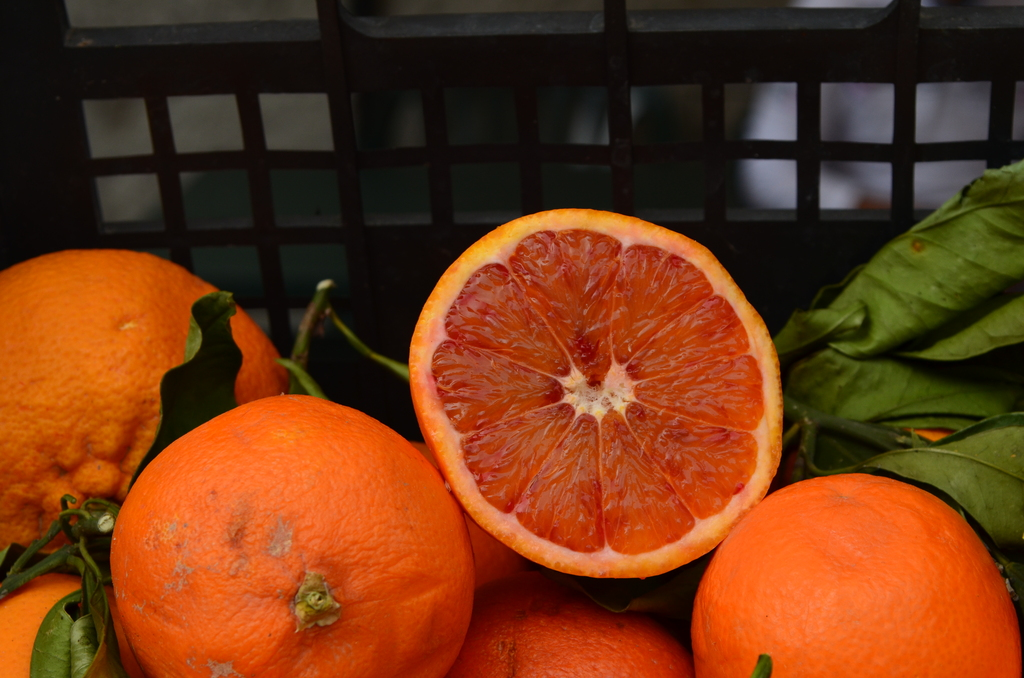
\includegraphics[width=0.8\textwidth]{Images/orangen.jpg}
		}{Bildquelle: Rune Knaak}
		\caption{Für die Platzierung ist bei diesem Bild die Option \code{[htbp!]} angegeben. Es wird daher von Latex dorthin geschoben, wohin es nach vorgegebenen Regeln passt. Mit der Option \code{[H]} würde das Bild ohne Rücksicht auf Schönheit genau an die Stelle gestellt, an der es im Latex-Text steht.}
	\label{fig:Platzhalter}
\end{figure}

Die Abbildung \ref{fig:Platzhalter} könnte auch eine Grafik zeigen, die mit einem externen Programm erzeugt wurde. Dabei werden die Formate PDF (*.pdf),
PNG (*.png), JPEG (*.jpg) und Encapsulated Postscript (*.eps) unterstützt.

Zu nicht selbst erstellten Bildern und Grafiken muss die Herkunft angegeben werden. Dafür eignet sich die Umgebung \verb|\copyrightbox{}|.

Es ist empfehlenswert, die Bilder in einem eigenen Unterordner zu sammeln -- zum Beispiel in einem Ordner \code{Images/}

Grafiken und Bilder sollten mit Bildunterschriften ausgestattet sein, die Auskunft darüber geben, was auf dem Bild zu sehen ist. Das wird mit dem Befehl \verb|\caption| innerhalb der figure-Umgebung erreicht.

Die Platzierung Bilder im Textfluss ist genau wie der Zeilenumbruch und allgemein die Verteilung des Inhalts auf eine Aufgabe von Latex. Dabei orientiert sich Latex an bestimmten harten Grundregeln, wie etwa der, dass Bilder nicht mit Text überlappen sollten und gewissen einprogrammierten Schönheitsregeln. So vermeidet Latex nach Möglichkeit große leere Bereiche. Die Priorität der Schönheitsregeln kann durch in eckigen Klammern gesetzten Optionen beeinflusst werden. Üblich ist dabei \code{[htbp!]}. Das steht für ``here", ``top", ``bottom" und ``page".

Mit der Option \code{[H]} kann man an dieser Stelle den Wunsch ausdrücken, das Bild genau an dieser Stelle in den Fließtext einzufügen. (Diese Option benötigt im Vorspann das Paket float)

Wenn keine Platzierung möglich erscheint, dann stellt Latex das betreffende Bild zurück. Dieses Bild ``blockiert" dann zunächst alle weiteren Bilder, denn Latex wird immer die Reihenfolge beibehalten. Im Ergebnis würden dann alle Bilder auf eigenen Seiten ganz hinten an das Dokument angehängt. Da das fast immer unerwünscht ist, ist im Vorspann zu diesem Dokument das Paket \code{[section]{placeins}} eingebunden. Es sorgt dafür, dass spätestens nach am Ende eines Abschnitts (\verb|\end{section}|) alle noch nicht platzierten Bilder und Tabellen ``abgeladen" werden.

Es gibt in Latex noch viele weitere Gestaltungsmöglichkeiten im Zusammenhang mit Bildern. Einen guten Überblick gibt dieses Kapitel im englischen Wikibook:
\begin{center}
	\url{https://en.wikibooks.org/wiki/LaTeX/Floats,_Figures_and_Captions}
\end{center}

\section{Tabellen erstellen}
Tabellen werden in Latex üblicherweise wie Bilder in einer verschiebbaren Umgebung angelegt. In diesem Fall handelt es sich um eine table-Umgebung (\verb|\begin{tabular}...\end{tabular}|). Die table-Umgebung enthält dann mit der tabular-Umgebung die eigentliche Tabelle und dazu mit \verb|\caption{}| die Tabellenunterschrift.

Die Darstellung von Tabellen kann man mit den Optionen und Parametern in vielfältiger Weise gestaltet werden. In der Tabelle \ref{tab:Rohdaten} wurden drei der besonders häufigen Bedürfnisse berücksichtigt:
\begin{itemize}
	\item Vereinigung von waagerecht nebeneinander liegenden Zellen\\
		$\Rightarrow$ Der Befehl \code{multicolumn{}{}{}}
	\item Ausrichtung der Werte auf das Dezimalkomma\\
		$\Rightarrow$ Formatierungskürzel \code{S}. Für diese Funktion wird das Paket siunitx gebraucht.
	\item Jede zweite Zeile wird leicht grau unterlegt\\
		$\Rightarrow$ Der Vorspann enthält den Befehl \verb|\rowcolors{1}{}{lightgray}| aus dem Paket xcolor.
\end{itemize}

Die meisten Latex-Umgebungen enthalten eine Funktion um den Rohbau einer Tabelle zu erstellen. Außerdem gibt es den Online-Service TablesGen, der recht viele Tabellenfunktionen kennt.\cite{TablesGen}).

\begin{table}[htbp!]
	\begin{center}
		\begin{tabular}{l|SSSSSSS}
			& \multicolumn{7}{c}{Versuchsläufe}              \\
			\rowcolor{white} & 1     & 2     & 3     & 4     & 5     & 6     & 7     \\
			\hline
			$t_1$ & 0,434 & 0,428 & 0,422 & 0,434 & 0,421 & 0,430  & 0,416 \\
			$t_2$ & 0,378 & 0,376 & 0,360  & 0,379 & 0,366 & 0,375 & 0,355 \\
			$t_3$ & 0,32  & 0,326 & 0,309 & 0,330  & 0,313 & 0,328 & 0,352 \\
			$t_4$ & 24,284 & 12,2   & 12,266 & 23,286 & 12,269 & 12,288 & 13,222
		\end{tabular}
		\caption{Messergebnisse. Gemessen wurden jeweils vier Zeiten zwischen aufeinander folgenden Stößen $t_i$. Die Messung wurde sieben Mal wiederholt.}
		\label{tab:Rohdaten}
	\end{center}
\end{table}

\section{Quellenangaben angeben}
Literaturverweise werden von Latex aus einer externen Datenquelle zusammen gesammelt. Im einfachsten Fall besteht diese Datenquelle aus einer Datei mit einer Reihe von Einträgen im Bibtex-Format. Für dieses Dokument hier ist dies die Datei \code{Literatur.bib}.

Der erste Parameter bei einem Eintrag im Bibtex-Format ist die Kennung unter der man ihn im Latex-Quelltext aufrufen kann. Dazu dient der Befehl \code{ref{}}. Dieser Befehl wird von latex gegen ein Kürzel ausgetauscht. Außerdem wird das Literaturverzeichnis um eine Langversion des Verweises erweitert.

Die Einträge aus der Datenquelle werden vom Hilfsprogramm \code{biber} eingesammelt und in eine für Latex lesbare Form gebracht (\code{*.bbl}, \code{*blg} und \code{*bcf}). Das heißt, dieses Programm muss vor dem Aufruf von Latex ausgeführt werden:
\begin{description}
	\item [Kile:] funktioniert automatisch ohne Konfiguration, kein eigener Aufruf nötig.
	\item [TeXmaker:] Options $\rightarrow$ Configure Texmaker $\rightarrow$ Commands $\rightarrow$ Bib(la)tex: \code{biber \%} \\
		Aufruf mit F11.
	\item [TeXstudio:] Options $\rightarrow$ Configure TeXstudio $\rightarrow$ Build $\rightarrow$ Default Bibliography Tool $\rightarrow$ biber \\
		Aufruf mit F8.
	\item [TeXworks:] Im Menü Typeset den Punkt ``biber" auswählen und ausführen.
\end{description}
Der Befehl \verb|\printbibliography| stellt das Literaturverzeichnis im fertigen Dokument dar.

\section{Formeln setzen}
Der Formelsatz von Latex ist exzellent. Von \$-Zeichen umgeben werden Formeln direkt in den Fließtext gesetzt: $\alpha = \beta + \Delta$. Um Formeln in einer eigenen Zeile abgesetzt darzustellen, nutzt man die equation-Umgebung
(\verb|\begin{equation}...\end{equation}|):
\begin{equation}
	e^{i \pi} + 1 = 0 \label{euler}
\end{equation}
Die Gleichung \ref{euler} wurde unsichtbar mit \verb|\label{euler}| markiert. Damit kann im Fließtext der Befehl \verb|\ref{euler}| auf die Gleichungsnummer  verweisen.

Wenn eine Nummerierung der Gleichung nicht gewünscht ist, hilft die Sternchen-Variante der equation-Umgebung (\verb|\begin{equation*}...\end{equation*}|):
\begin{equation*}
	\langle X\rangle =\frac{1}{N}\sum\limits_{i=1}^{N}X_i
\end{equation*}

\section{Werte darstellen}
Durch Messungen ermittelte Werte haben meist eine Einheit und eine Unsicherheit. Um dies korrekt darzustellen, eignet sich der Befehl \code{SI{}{}} aus dem Paket siunitx. Die Eingabe ist recht flexibel. Der Befehl erkennt verschiedene Notationen für die Unsicherheit. Beispiele:
\begin{itemize}
	\item \verb|\SI{3.14(4)}{m \per \second^{2}}| \hfill $\rightarrow$ \hfill
		\SI{3.14(4)}{m \per \second^{2}}
	\item \verb|\SI{3.14 +- 0,04}{\kilogram \metre \per \second}| \hfill $\rightarrow$ \hfill
		\SI{3.14 +- 0,04}{\kilogram \metre \per \second}
\end{itemize}
Die Formatierung der Ausgabe lässt sich konfigurieren. Wie sehr das ins Detail geht, kann man daran ablesen, dass die Dokumentation des Pakets 96 Seiten umfasst:
\begin{center} \url{http://mirrors.ctan.org/macros/latex/contrib/siunitx/siunitx.pdf} \end{center}

\section{Das Deckblatt}
Ein Versuchsbericht ist erst mit dem Deckblatt des Physikpraktikums fertig für eine Abgabe. Seit Herbst 2020 ist das Deckblatt als PDF-Formular mit Textfeldern zum nachträglichen, digitalen Ausfüllen gestaltet. Leider gehen diese ausfüllbaren Textfelder bei der Einbindung eines PDFs  innerhalb von Latex verloren. Deshalb wird das Deckblatt in dieser Vorlage als Latex-Code mit Hilfe des Befehls \verb|input{}| eingebunden.

Alternativ können Sie das PDF des Deckblatts nachträglich mit einem getrennten Programm vor das von Latex erstellte PDF setzen. Für diese Aufgabe eignet sich \verb|pdfunite|. Dieses Hilfsprogramm ist Teil der freien Bibliothek \href{http://poppler.freedesktop.org/}{Poppler}, die sowohl bei TeXlive als auch bei MikTex mitgeliefert wird. Aufruf in der Kommandozeile:
\begin{itemize}
	\item \verb|pdfunite Deckblatt.pdf BERICHT.pdf BERICHT_MIT_DECKBLATT.pdf|
\end{itemize}
Das Programm \verb|pdfsam| erfüllt die gleiche Funktion mit einer grafischen Bedienoberfläche. Es ist für Linux in vielen Distributionen enthalten. Für Windows und MacOS ist es auf der \href{https://pdfsam.org/download-pdfsam-basic/}{Downloadseite des Projekts} erhältlich.

\section{Die Quelldateien dieses Dokuments}
Das PDF dieses Dokuments benötigt zur Erstellung die folgenden Dateien:
\begin{itemize}
	\item \code{Versuchsbericht-latex.tex}
	\item \code{Vorspann.tex}
	\item \code{Deckblatt-Formular.tex}
	\item \code{Deckblatt-Vorspann.tex}
	\item Unterordner \code{Images} mit den Bildern \code{ap-logo\_bw.pdf} und \code{orangen.jpg}
\end{itemize}
Andere Dateien, die Sie möglicherweise in dem Ordner des Dokuments finden, wurden von Latex automatisch erstellt. Sie können sie ohne Schaden löschen. Bei Bedarf werden die Dateien beim nächsten Lauf von pdflatex oder biber wiederhergestellt.


\section{Zusammenfassung}
Das Satzsystem \LaTeX{} eignet sich gut zur Erstellung von Versuchsberichten im Physikpraktikum. Es gibt für Latex eine Auswahl an Umgebungen, die für unterschiedliche Arbeitsweisen ausgerichtet sind. Formeln werden perfekt dargestellt. Mit anderen Werkzeugen erstellte Grafiken und Fotos können als PDF eingebunden werden.
\footnote{Am Ende des Versuchsberichts steht die Zusammenfassung. Die Zusammenfassung fasst die wichtigsten Ergebnisse aus dem Hauptteil des Berichts in einer Handvoll Zeilen zusammen. Sie präsentiert keine neuen Ergebnisse.}

\clearpage % Quellenangaben auf einer neuen Seite
\printbibliography
\end{document}
